\begin{frame}
  \frametitle{Sparse Grids -- Basics}
  \topline
  \vspace{-10px}
  \begin{block}{Hierarchical Basis}
    \begin{figure}[!htp]
      \setbeamertemplate{caption}{\raggedright\insertcaption\par}
      \setbeamerfont{caption}{size=\footnotesize}
      \centering
      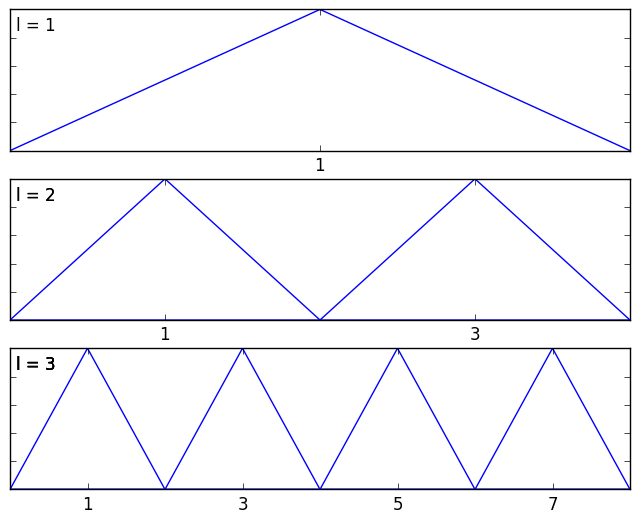
\includegraphics[width=7.5cm]{images/sparse_hats}
      \vspace{-12px}
      \caption{}
    \end{figure}
  \end{block}
\end{frame}

\begin{frame}
  \frametitle{Sparse Grids -- Basics}
  \topline
  \vspace{-10px}
  \begin{block}{Hierarchical basis (vs nodal basis)}
    \begin{itemize}
      \item Grouping grid points into levels $l \in \{1,2,3\dots , n\}$
      \item Basis function by index \textbf{and} level: $\phi_{l,i}(x)$
    \end{itemize}
    \vspace{20px}
      $$\hat{f}(x) = \sum_{l \leq n,i \in G_l}{\ \alpha_{l,i} \cdot \phi_{l,i}(x)}$$
  \end{block}
\end{frame}

\begin{frame}
  \frametitle{Sparse Grids -- Basics}
  \topline
  \vspace{-10px}
  \begin{block}{Hierarchical Basis}
    \begin{figure}[!htp]
      \setbeamertemplate{caption}{\raggedright\insertcaption\par}
      \setbeamerfont{caption}{size=\footnotesize}
      \centering
      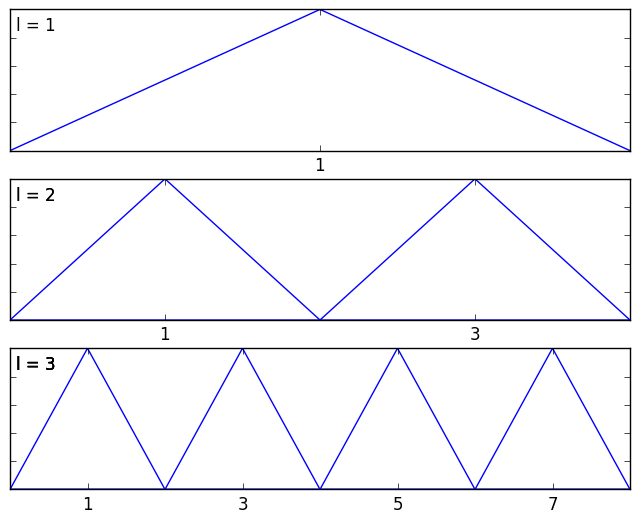
\includegraphics[width=7.5cm]{images/sparse_hats}
      \vspace{-12px}
      \caption{}
    \end{figure}
  \end{block}
\end{frame}

\begin{frame}
  \frametitle{Sparse Grids -- Basics}
  \topline
  \vspace{-10px}
  \begin{block}{Hierarchical vs. nodal basis}
    \begin{figure}[!htp]
      \setbeamertemplate{caption}{\raggedright\insertcaption\par}
      \setbeamerfont{caption}{size=\footnotesize}
      \centering
      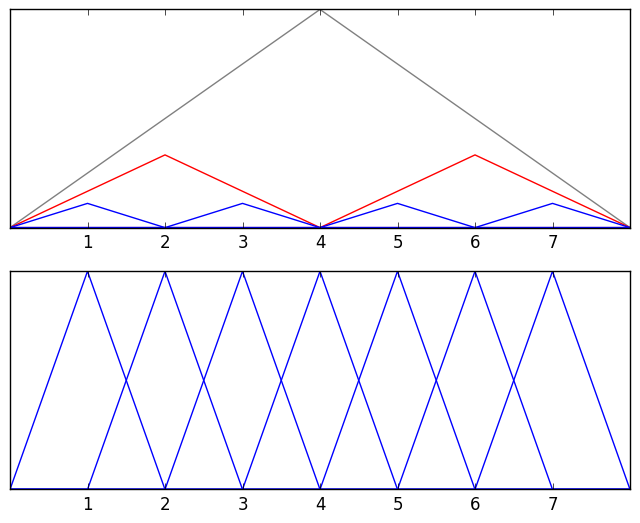
\includegraphics[width=7.5cm]{images/sparse_together}
      \vspace{-12px}
      \caption{}
    \end{figure}
  \end{block}
\end{frame}

\begin{frame}
  \frametitle{Sparse Grids -- Basics}
  \topline
  \vspace{-10px}
  \begin{block}{Full grid discretization: Hierarchical basis}
    \begin{figure}[!htp]
      \setbeamertemplate{caption}{\raggedright\insertcaption\par}
      \setbeamerfont{caption}{size=\footnotesize}
      \centering
      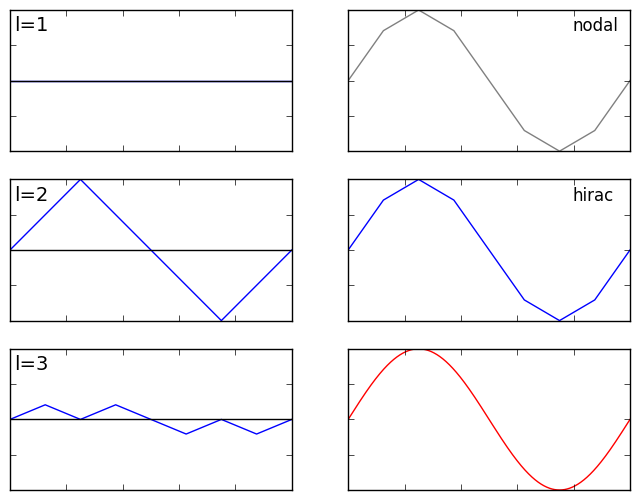
\includegraphics[width=7.5cm]{images/sparsegrid_1d_1}
      \vspace{-12px}
      \caption{}
    \end{figure}
  \end{block}
\end{frame}


\begin{frame}
  \frametitle{Sparse Grids -- Basics}
  \topline
  \vspace{-10px}
  \begin{block}{Full grid discretization: Hierarchical basis}
    \begin{figure}[!htp]
      \setbeamertemplate{caption}{\raggedright\insertcaption\par}
      \setbeamerfont{caption}{size=\footnotesize}
      \centering
      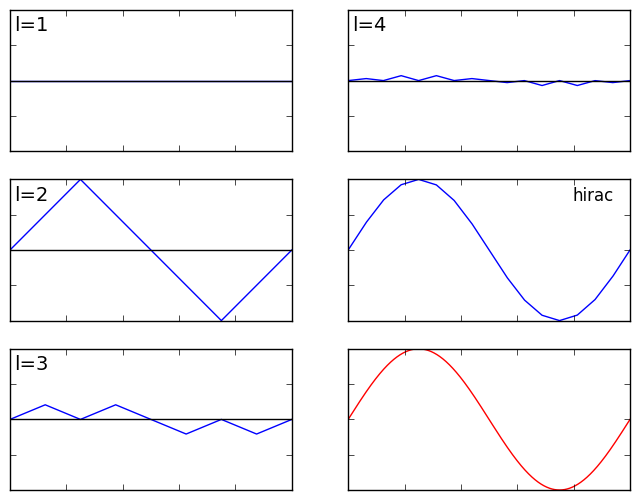
\includegraphics[width=7.5cm]{images/sparsegrid_1d_2}
      \vspace{-12px}
      \caption{}
    \end{figure}
  \end{block}
\end{frame}

\begin{frame}
  \frametitle{Sparse Grids -- Basics}
  \topline
  \vspace{-10px}
  \begin{block}{Basis function subspaces}
    \begin{itemize}
      \item Combination of levels and dimensions
      \item Notion of hierarchical subspaces
      \item Defined by the levels of detail in all dimensions $(l_x, l_y, ...)$
    \end{itemize}
  \end{block}
\end{frame}

\begin{frame}
  \frametitle{Sparse Grids -- Basics}
  \topline
  \vspace{-10px}
  \begin{block}{Hierarchical grid points}
    \begin{figure}[!htp]
      \setbeamertemplate{caption}{\raggedright\insertcaption\par}
      \setbeamerfont{caption}{size=\footnotesize}
      \centering
      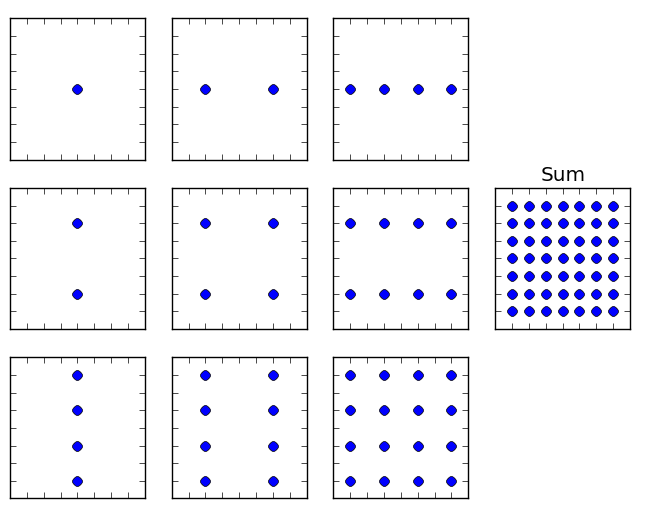
\includegraphics[width=7.5cm]{images/sparsegrid_hirach1}
      \vspace{-12px}
      \caption{}
    \end{figure}
  \end{block}
\end{frame}

\begin{frame}
  \frametitle{Sparse Grids -- Basics}
  \topline
  \vspace{-10px}
  \begin{block}{Hierarchical subspaces}
    \begin{figure}[!htp]
      \setbeamertemplate{caption}{\raggedright\insertcaption\par}
      \setbeamerfont{caption}{size=\footnotesize}
      \centering
      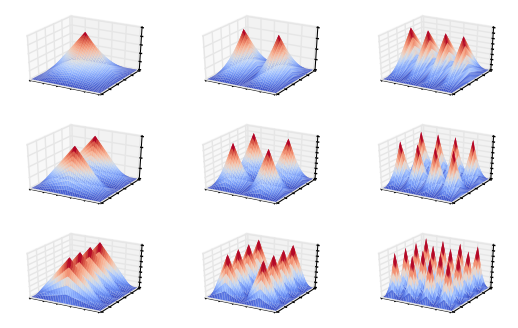
\includegraphics[width=7.5cm]{images/sparsegrid_2dhats}
      \vspace{-12px}
      \caption{}
    \end{figure}
  \end{block}
\end{frame}

\begin{frame}
  \frametitle{Sparse Grids -- Basics}
  \topline
  \vspace{-10px}
  \begin{block}{Sparse grid -- Changes}
    \begin{itemize}
      \item Throwing away certain subspaces
      \item Finding those is a \emph{a-priori} solvable optimization problem
      \item The resulting grid is now \textbf{sparse}
      \end{itemize}
  \end{block}
  \begin{block}{Profit}
    \begin{itemize}
      \item Reducing the computational effort ``a lot''
      \item Maintaining ``high'' accuracy
      \end{itemize}
  \end{block}
\end{frame}

\begin{frame}
  \frametitle{Sparse Grids -- Basics}
  \topline
  \vspace{-10px}
  \begin{block}{A \emph{sparse} grid}
    \begin{figure}[!htp]
      \setbeamertemplate{caption}{\raggedright\insertcaption\par}
      \setbeamerfont{caption}{size=\footnotesize}
      \centering
      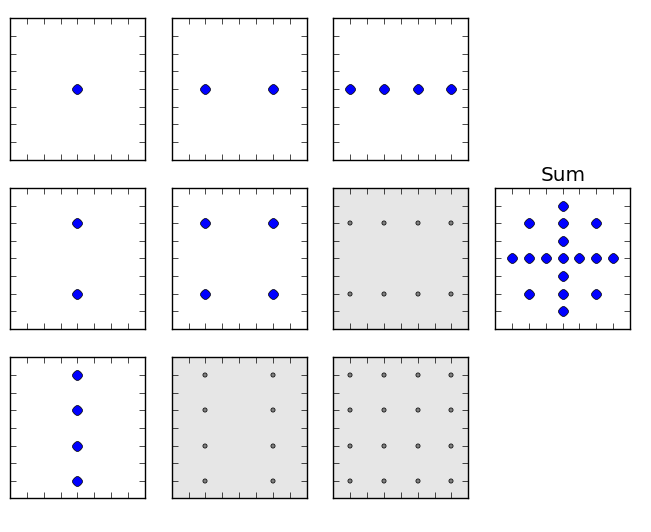
\includegraphics[width=7.5cm]{images/sparsegrid_hirach2}
      \vspace{-12px}
      \caption{}
    \end{figure}
  \end{block}
\end{frame}

\begin{frame}
  \frametitle{Sparse Grids -- Basics}
  \topline
  \vspace{-10px}
  \begin{block}{Boundary and smoothness}
    \begin{itemize}
      \item Boundaries need special treatment
      \item The function needs to be sufficiently smooth \\
        $D^2f$ needs to be bounded
      \end{itemize}
  \end{block}
  \begin{block}{Adaptivity}
    \begin{itemize}
      \item \emph{A-posteriori} modifications to better fit the function
      \item Picking a single grid point and adding level of detail around it
      \item Prone to overfitting and huge computational effort
      \end{itemize}
  \end{block}
\end{frame}


\begin{frame}
  \frametitle{Sparse Grids -- Basics}
  \topline
  \vspace{-10px}
  \begin{block}{Summary}
    \begin{itemize}
      \item Hierarchical basis through grouping grid points into levels
      \item Creating ``subspaces'' through combination of levels in dimensions
      \item Selecting and combining subspaces
      \end{itemize}
  \end{block}
  \begin{block}{To keep in mind}
    \begin{itemize}
      \item Smoothness requirement for $f(x)$
      \item Boundary treatment
      \item Accuracy--effort trade-off
      \item Adaptivity options (\emph{a-posteriori})
      \end{itemize}
  \end{block}
\end{frame}

%%% Local Variables:
%%% TeX-master: "slides"
%%% End:
